\documentclass[11pt]{article}
\usepackage[margin=1in]{geometry}
\usepackage[T1]{fontenc}
\usepackage{lmodern}
\usepackage{microtype}
\usepackage{graphicx}
\usepackage{booktabs}
\usepackage{tabularx}
\usepackage{array}
\usepackage{xcolor}
\usepackage[most]{tcolorbox}
\usepackage{enumitem}
\usepackage[hidelinks]{hyperref}
\usepackage{titlesec}
\usepackage{float}

\definecolor{accent}{HTML}{2a78d6}
\definecolor{hard}{HTML}{eb6834}
\definecolor{muted}{HTML}{52514e}
\definecolor{boxbg}{HTML}{f3f6fb}
\titleformat{\section}{\large\bfseries}{\thesection}{0.6em}{}
\titleformat{\subsection}{\normalsize\bfseries}{\thesubsection}{0.6em}{}
\setlist{itemsep=2pt, topsep=3pt}
\newcolumntype{L}{>{\raggedright\arraybackslash}X}
\renewcommand{\arraystretch}{1.25}

\newtcolorbox{hyp}[1]{colback=boxbg, colframe=accent, boxrule=0.8pt, arc=2pt,
  left=8pt, right=8pt, top=6pt, bottom=6pt, fonttitle=\bfseries, title=#1}
\newtcolorbox{verdict}{colback=white, colframe=muted!40, boxrule=0.5pt, arc=2pt,
  left=6pt, right=6pt, top=4pt, bottom=4pt}

\begin{document}

\begin{center}
{\LARGE\bfseries Out of Sight, Out of Plan}\\[4pt]
{\large Compact latent world models drop the objects a later task needs}\\[10pt]
{\normalsize Research proposal with preliminary results \quad$\cdot$\quad Rishi Simhadri \quad$\cdot$\quad October 7, 2026}
\end{center}

\vspace{4pt}
\begin{tcolorbox}[colback=white, colframe=muted!30, boxrule=0.5pt, arc=2pt, left=8pt, right=8pt]
\textbf{In one paragraph.} Latent world models such as LeWM compress each camera frame into a short vector and plan by searching for actions whose \emph{predicted} vector lands close to the vector of a goal image. We asked what survives that compression when a task needs an object the model was not built around. In a controlled PushT variant with a second, movable object (a ``peg''), LeWM moves the familiar T-block to its goal in 49--74\% of scenes but moves the peg to its goal in only \textbf{1--3\%}. A planner with access to the true physics solves both tasks about \textbf{99\%} of the time. The failure is not explained by task difficulty, object size, lack of training exposure, or training length: the peg is simply \textbf{absent from the model's representation}. Strikingly, forcing the peg into the representation with privileged labels \emph{still} leaves planning at 1\%, which points to a second failure in how goals are scored. Peg-moving stays at 0--3\% in every model we evaluated, and the gap survives every alternative explanation we tested.
\end{tcolorbox}

\section{Motivation}

A world model lets a robot ``imagine'' the result of an action before taking it. Recent \emph{latent} world models skip predicting pixels: they encode each image into a compact vector and learn to predict the next vector. LeWM, the model we study, encodes a whole $224\times224$ image into \textbf{one vector of 192 numbers}. For comparison, DINO-WM keeps about 75{,}000 numbers per frame. To plan, LeWM samples many candidate action sequences, predicts where each one leads, and picks the sequence whose predicted vector is \emph{closest} to the goal image's vector.

Compression forces a choice about what to keep, and the model makes that choice during training, before it knows which tasks it will face. Relevance, however, belongs to the task rather than to the object. The same cup can be clutter in one task, an obstacle in another, and the target in a third. A representation tuned to its training data may therefore silently discard exactly the object a later task depends on. If it does, no amount of planning can recover it, because the planner only ever sees the compressed vector.

This question matters beyond one model. Compact latents are attractive because they make planning fast (LeWM plans up to $48\times$ faster than foundation-feature world models), and the field is moving toward them. Whether compact world models keep \emph{the information decisions need} is therefore a general concern. The concern extends past a single benchmark score.

\section{Hypothesis}

\begin{hyp}{Main hypothesis (H)}
A compact latent world model trained with a predictive objective keeps the objects that dominate its training dynamics and discards other objects in the scene. As a result, a planner that uses the model \textbf{cannot achieve goals that depend on those other objects}, even when they are clearly visible, comparable in size to the main object, and frequently moved in the training data.
\end{hyp}

\noindent The hypothesis makes concrete, falsifiable predictions. If H is true:
\begin{enumerate}[label=\textbf{P\arabic*.}]
  \item In identical scenes, the model succeeds at goals about the familiar object but fails at matched goals about the second object, while a planner with true physics solves both equally well.
  \item The second object's position cannot be read out of the model's vector, even though it is easy to read from the raw pixels.
  \item The failure persists when the object is made large, when it is pushed often in training data, and when training runs longer.
\end{enumerate}
H would be \emph{false} if any of these hold: the reference planner also fails (the task is just hard); enlarging the object fixes it (it is only about size); frequent exposure or longer training fixes it (it is only missing data or training); or the object's position is readable from the vector (the information is there and the problem lies elsewhere).

\noindent A refinement emerged from the results (Section~\ref{sec:fixes}):

\begin{hyp}{Refined hypothesis (H$'$): a two-layer failure}
\textbf{Layer 1 (representation):} the encoder drops the secondary object. \\
\textbf{Layer 2 (planning objective):} even when the object is put back into the vector, scoring plans by overall distance to the goal vector does not make use of it, so planning still fails.
\end{hyp}

\section{Experimental setup}

\paragraph{Environment: PushT-Peg.} We extended the standard PushT task (a round pusher moves a T-shaped block) with one extra movable disc, the \emph{peg} (Figure~\ref{fig:env}). The peg is orange, distinct from the blue pusher and gray T. It has radius 15 by default (about 13 pixels across in the model's $224\times224$ input) and radius 45 in a size control (similar in scale to the T).

\begin{figure}[h]
\centering
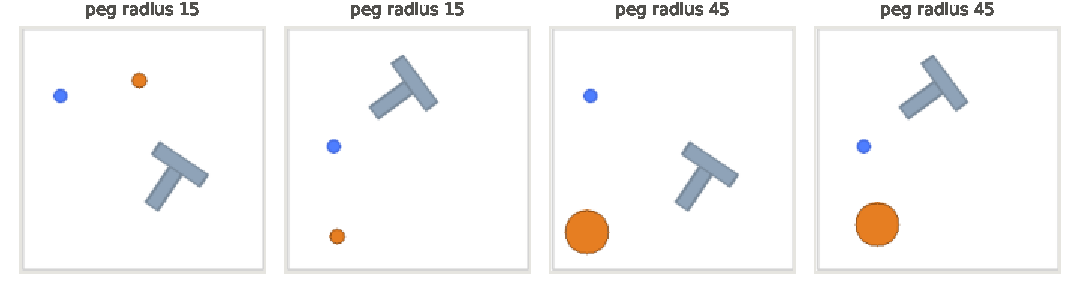
\includegraphics[width=\linewidth]{figures/env.pdf}
\caption{PushT-Peg scenes. Blue: pusher. Gray: T-block. Orange: peg (left two: default radius 15; right two: radius 45 size control).}
\label{fig:env}
\end{figure}

\paragraph{Models.} All models share LeWM's architecture and objective (predict the next 192-number vector, plus a regularizer that keeps vectors spread out).
\begin{itemize}
  \item \textbf{Pretrained LeWM}: the published checkpoint, trained on PushT data with no peg.
  \item \textbf{Peg-as-clutter} (2 seeds): fine-tuned from the pretrained model on PushT-Peg data where the pusher works on the T and the peg sits off to the side. The peg is touched in 2.9\% of frames.
  \item \textbf{Peg-pushed (``mixed'')} (2 seeds): fine-tuned on data where half the episodes deliberately push the peg. The peg is touched in 37\% of frames.
\end{itemize}
Both training sets share the same scenes and peg placement; only the data-collection policy differs. Fine-tuning used upstream's settings (2,000 steps, batch 128, bf16) on a rented H100.

\paragraph{Test conditions.} Each test scene starts from a real trajectory with the pusher already near the object to be moved (as in LeWM's own evaluation). From the same scene we build matched goals:
\begin{center}
\begin{tabularx}{\linewidth}{@{}lL@{}}
\toprule
Condition & What the goal asks \\
\midrule
\textbf{move the T} & move the T-block a set distance; leave the peg alone (control) \\
\textbf{move the peg} & move the peg the \emph{same} distance; leave the T alone (target role) \\
\textbf{peg away from path} & move the T; the peg sits far from its path (control) \\
\textbf{peg beside path} & move the T; the peg sits 55\,px beside its path and must not be disturbed (don't-disturb role) \\
\bottomrule
\end{tabularx}
\end{center}

\paragraph{Fair yardstick.} A \textbf{reference planner} uses the same search procedure but simulates candidates with the true physics. A scene counts only if the reference solves both goals of a comparison. This filter ensures that a gap reflects the model rather than an impossible task.

\paragraph{Measurements.}
\begin{itemize}
  \item \textbf{Planning success}: whether the object reaches its goal within 50 steps.
  \item \textbf{Readout}: how well an object's position can be recovered from the model's vector, measured as error in pixels. The two reference points are the error of always guessing the average position (no information) and the error of reading the raw pixels (what is available in the image).
  \item \textbf{Candidate-ranking analysis (A/B/C)}: separates prediction errors from representation and scoring errors.
\end{itemize}
Every decision rule was written down before results were seen. The main run used 400 scenes per model and condition: 8,000 model episodes and 3,200 reference episodes.

\section{Main result}

\begin{figure}[h]
\centering
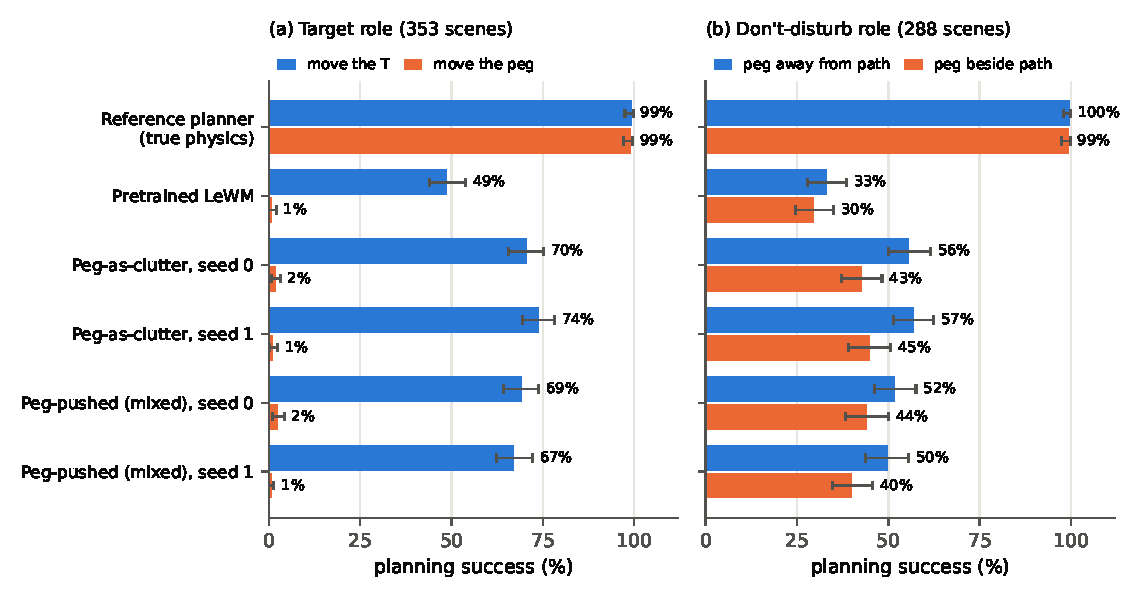
\includegraphics[width=\linewidth]{figures/success.pdf}
\caption{Planning success on scenes the reference planner can solve, with 95\% confidence intervals. \textbf{(a)}~Every LeWM model can move the T but essentially never the peg, while the reference does both. \textbf{(b)}~The don't-disturb gap is smaller (7--13 points).}
\label{fig:success}
\end{figure}

\noindent\textbf{Target role (Figure~\ref{fig:success}a).} The gap between moving the T and moving the peg is \textbf{48 points for the pretrained model and 67--73 points for every fine-tuned model}. The confidence intervals are about $\pm5$ points, and the reference planner shows no gap ($-0.3$ points). Fine-tuning improved T-moving (49\% $\to$ 67--74\%) but left peg-moving at the floor, including for the models trained on data where the peg is pushed constantly.

\noindent\textbf{Don't-disturb role (Figure~\ref{fig:success}b).} Peg-as-clutter models score 12--13 points lower when the peg sits beside the path (intervals exclude zero). This falls just short of our pre-set 15-point bar. The T-only success barely changes (3--4 points), so the drop comes from bumping the peg. The peg-pushed models narrow it to 8--10 points.

\section{Ruling out alternative explanations}
\label{sec:fixes}

Table~\ref{tab:alts} summarizes the tests. Each alternative makes a prediction that differs from H, and each was tested with an outcome rule fixed in advance.

\begin{table}[!htb]
\centering
\small
\begin{tabularx}{\linewidth}{@{}>{\raggedright\arraybackslash}p{3.4cm}L>{\raggedright\arraybackslash}p{4.1cm}>{\raggedright\arraybackslash}p{1.9cm}@{}}
\toprule
Alternative explanation & Test & Result & Ruled out? \\
\midrule
1. The peg task is just harder & Reference planner with true physics on identical scenes & 99\% (peg) vs 99\% (T) & \textbf{Yes} \\
2. The model never saw the peg move & Train on data where the peg is pushed in 37\% of frames & Peg success 1--2\%, gap 67--73 pts & \textbf{Yes} \\
3. The peg is too small to see & Enlarge peg to T scale (radius 45), at test time and with retraining & Peg success 1--3\%; readout at guessing level & \textbf{Yes} \\
4. Not enough training & Fine-tune 5$\times$ longer (10,000 steps) & Peg success 0/85, gap 73 pts & \textbf{Yes}$^\dagger$ \\
5. Information is there, just not linearly readable & Nonlinear (MLP) and nearest-neighbor readouts & At guessing level in all 28 cases & \textbf{Yes} \\
6. A published fix already solves it & Inverse-dynamics loss (arXiv 2610.03137) & Peg success 1\%; T success drops to 24\% & \textbf{Yes} \\
7. Missing information is the whole story & Train with privileged peg-position labels & Peg now readable (19\,px) but success still 1\% & \textbf{No}: a second bottleneck \\
\bottomrule
\end{tabularx}
\caption{Alternatives and outcomes. $^\dagger$A from-scratch training arm meant to separate ``pretraining lock-in'' from ``objective'' failed to become competent (8\% even on the T) and is uninformative.}
\label{tab:alts}
\end{table}

\subsection*{1.\ Is the peg task harder? \textmd{No.}}
The reference planner, which searches with the true physics, succeeds 98.9\% on peg goals and 99.2\% on matched T goals (353 scenes). Both goals are equally reachable within the same step budget for a planner that can see the peg.

\subsection*{2.\ Is it lack of exposure? \textmd{No.}}
The peg-pushed models were trained on data in which the peg is in contact with the pusher in 37\% of frames (13$\times$ more than the clutter models). They still move the peg to its goal only 1--2\% of the time. By our pre-set rule, the mixed data counts only as ``reduced disparity'' on the don't-disturb task and gives no improvement on the target task.

\begin{verdict}
\small Prediction P3 (exposure) holds: exposure does not teach the model to represent or plan with the peg.
\end{verdict}

\subsection*{3.\ Is it just object size? \textmd{No.}}
At radius 15 the peg covers less than one of the model's $14\times14$ input patches, so size was a serious candidate. We tested it in two stages.
\begin{itemize}
  \item \textbf{Test time.} Enlarging the peg to radius 45 makes it trivially readable from raw pixels (14.5\,px error), yet readout from every fine-tuned model's vector stays at the level of guessing (0.98--1.02$\times$ the guessing error). The T is read to 19--27\,px.
  \item \textbf{Retraining on big-peg data.} The models still move the peg only 1--3\% of the time, versus 54--68\% for the T, with gaps of 53--64 points. The reference planner shows no gap at this size ($-2$ points).
\end{itemize}

\subsection*{4.\ Is it too little training? \textmd{No (for fine-tuning).}}
Fine-tuning 5$\times$ longer on the peg-pushed data lowered prediction error until it plateaued, and slightly improved T-moving (67\% $\to$ 73\%). Peg-moving fell to 0 of 85 scenes, and peg readout stayed at guessing level (0.88$\times$). A model trained from scratch overfit the smaller dataset and could not plan even with the T (8\%). We therefore cannot yet separate ``locked in by pretraining'' from ``caused by the objective itself''.

\subsection*{5.\ Is the peg present but hard to decode? \textmd{No.}}
Linear, nonlinear (MLP) and nearest-neighbor readouts all locate the peg no better than guessing, in all 28 combinations of model, peg size and embedding (Figure~\ref{fig:readout}). The same nearest-neighbor readout recovers the T from the same vectors, and the peg from coarse raw pixels. The information is in the image and lost in the vector.

\begin{figure}[h]
\centering
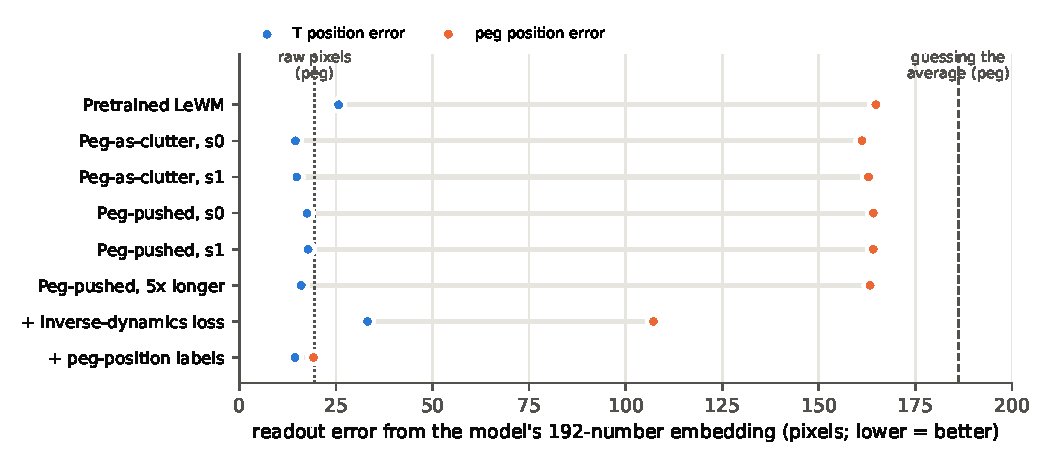
\includegraphics[width=0.92\linewidth]{figures/readout.pdf}
\caption{How well the T (blue) and the peg (orange) can be located from each model's 192-number vector (linear readout, radius 15, same frames for every model). Every standard model reads the T well and the peg at the guessing level. Only privileged peg labels put the peg into the vector.}
\label{fig:readout}
\end{figure}

\subsection*{6--7.\ Does a known fix work, and is missing information the whole story?}
We tested two training-time additions, each on the peg-pushed data under the same recipe.
\begin{itemize}
  \item \textbf{Inverse-dynamics loss.} This is the fix from the closest prior work, \emph{Keeping JEPA World Models Plannable When Little of the Frame Moves} (arXiv 2610.03137), matched to its published form and weights. It partly improved peg readout (164 $\to$ 107\,px) but did not enable peg-moving (1\%). With these weights it also damaged the model's predictions, and T-moving fell to 24\%.
  \item \textbf{Privileged peg-position labels} (an upper bound, since it uses information a general method would not have). The peg became fully readable from the vector (19\,px, as good as raw pixels), yet peg-moving stayed at \textbf{1\%}.
\end{itemize}
This last result is the most informative. Restoring the information does not restore planning. The candidate-ranking analysis agrees: on peg goals, even \emph{real} outcomes encoded by the model rank candidates worse than on T goals (rank correlation 0.58 vs 0.75). The goal-distance score is therefore dominated by the T and the pusher, and it barely moves when the peg moves.

\begin{verdict}
\small Predictions P1--P3 hold, so H is supported. The privileged-label result shows the failure has a \textbf{second layer}: the planning objective. This motivates the refined hypothesis H$'$.
\end{verdict}

\section{What this means}

\begin{enumerate}
  \item \textbf{The hypothesis is supported, in a sharper form.} LeWM organizes its 192-number vector around the object that dominates its training and treats a second object as background. This holds even when the object is large, moves often, and matters for the goal. Size, exposure, training length, readout method and a published fix all fail to explain it away.
  \item \textbf{The failure has two layers.} The representation drops the object (Layer~1), and the standard way of scoring plans cannot use the object even when it is present (Layer~2). A better representation alone will therefore not be enough. Most related work targets only the representation.
  \item \textbf{The effect is large and robust.} Peg-moving success is 0--3\% in every one of the 10 models evaluated (pretrained plus 9 trained), against 49--74\% T-moving success for every model whose T planning was intact, across three evaluation rounds. A reference planner rules out task difficulty, and every outcome rule was set before seeing results.
\end{enumerate}

\section{Limitations}
\begin{itemize}
  \item \textbf{One environment and one model family.} The evidence comes from a single simulated 2-D task (PushT-Peg) and from LeWM only. Generality across environments and world models is untested.
  \item \textbf{Few training seeds.} The main run has two seeds per training arm, and the follow-up checks have one.
  \item \textbf{Reused scenes in the follow-ups.} The follow-up checks reuse the first 100 scenes of the main run, so they are exploratory rather than confirmatory.
  \item \textbf{Lock-in vs objective is unresolved.} The from-scratch arm was not competent, so it could not decide between the two.
  \item \textbf{The inverse-dynamics comparison is imperfect.} We fine-tuned rather than trained from scratch as the paper did, and the paper's weights dominated our loss.
  \item \textbf{Close prior work.} Related work reports LeWM-style blindness to parts of a scene (arXiv 2610.03137; StarWM's passive-object analysis; ``representation laziness'' in Spectral-Target). Our distinct contributions are the matched role-swap test with a fair reference, the systematic elimination of alternatives, and the finding that restoring the information does not restore planning.
\end{itemize}

\section{Significance and proposed question}

\paragraph{Where this stands.} The current evidence supports a solid \textbf{workshop paper}: a clean, well-controlled diagnostic of a large failure in compact latent world models, plus a surprising negative result for an existing fix and for privileged supervision. Main-conference strength would require showing that the effect generalizes beyond LeWM on PushT, and ideally a general, label-free remedy that addresses both layers.

\noindent\textbf{Proposed research question.}\par\vspace{2pt}
\begin{hyp}{Question}
How can a compact latent world model keep, \emph{and plan with}, objects whose relevance only appears at test time, without knowing the task or naming the objects in advance?
\end{hyp}

\vspace{6pt}
\noindent{\sloppy\small\color{muted} Reproducibility: code and pre-registered protocol on branch \texttt{research/role-swap-probe} of \url{https://github.com/rishisim/lewm-p2-contact}; results in \url{experiments/role_swap/results/}. Total GPU cost for all training $\approx$\$11.50.\par}

\end{document}
